\documentclass[12pt,a4paper]{article}

\usepackage[dvipsnames]{xcolor}
\usepackage{amsmath}
\usepackage{amsfonts}

\usepackage{tikz}
\tikzset{every picture/.style={line width=0.75pt}} %set default line width to 0.75pt        
\newcommand{\pard}[2]{\frac{\partial #1}{\partial #2}}
\begin{document}
	
\begin{center}	
	
	\huge{Shape optimization of a magmatic body} \\ 
	 \vspace{1cm}
	\Large{June 2024 \\ 
	Théo Perrot}
\end{center}


\section{Introduction}

To understand the internal structure of a volcano, one can use the surface displacement field as a proxy for the underlying magmatic processes. 

Such a displacement field can be acquired by various mehods, the most used nowadays being the GNSS (Global Navigation Satellite System) point measurement and the InSAR (Interferometric Synthetic Aperture Radar) far-field measurement. In brief, the first consist in a station fixed to the ground which measure to a millimeter scale its position in a global reference frame. A good temporal precision can be achieved (1 point every 8 hours) but this method yield only the spatial position of point. On the other hand, InSAR measurements can cover a large area but with poor temporal resolution. This is achieved using a taking the phase difference of two successive phase image taken from the same position by a satellite flying over the area. Knowing the wavelength of the wave sent, the phase difference can be turned in a change in the position of the ground. These two kind of measurements can be then merged into a smooth displacement map thanks to physics-based interpolation methods.

Assuming a pressurized magmatic body is responsible for the inflation, we aim to know its characteristics : its location, its depth, its internal pressure and its shape. Many approaches are implemented in the literature to solve this inverse problem, but all of them are assuming a predefined parametrized shape for the magmatic body (like a sphere or an ellipsoid).

Here, we are trying to implement a shape optimization approach to explore new, unparametrized shapes that could explain the observed displacement field.

\section{Problem}

Practically, we model a domain representing a portion of the shallow earth crust including the volcano, see Fig. \ref{mod}.

The goal is then to use a shape optimization algorithm to seek for the most likely shape for the magma chamber, but instead of minimizing the compliance as it is often the case, the objective function to minimize would be the error between the observed and the computed surface displacement. 

\begin{figure}[h]
	
	
	\centering
	
	
	
	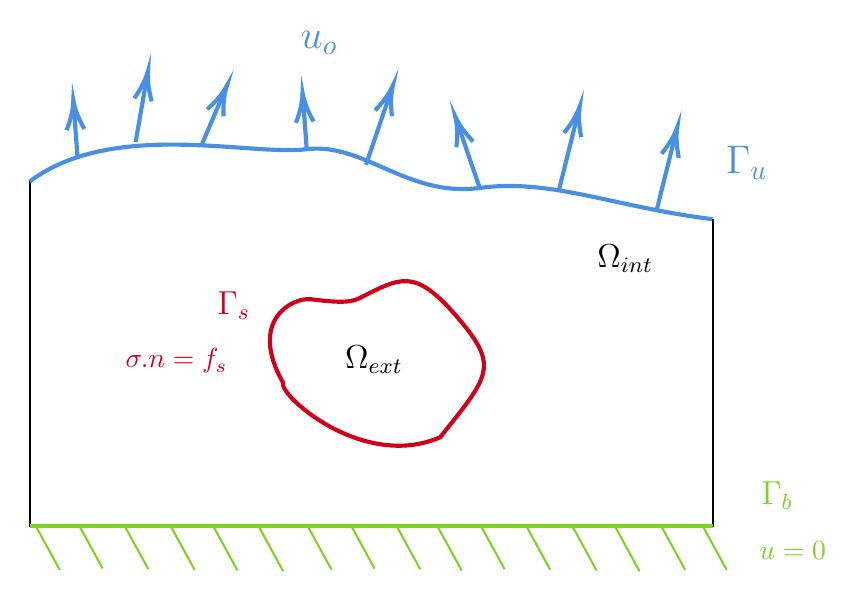
\begin{tikzpicture}[x=0.75pt,y=0.75pt,yscale=-1,xscale=1]
		%uncomment if require: \path (0,332); %set diagram left start at 0, and has height of 332
		
		%Shape: Right Angle [id:dp5784111444422806] 
		\draw  [color={rgb, 255:red, 0; green, 0; blue, 0 }  ,draw opacity=1 ] (509,268.39) -- (212,268.39) -- (212,102.22) ;
		%Curve Lines [id:da7656569557638543] 
		\draw [color={rgb, 255:red, 74; green, 144; blue, 226 }  ,draw opacity=1 ][line width=1.5]    (212,102.22) .. controls (252,72.22) and (318,90.06) .. (345.44,86.67) .. controls (372.89,83.28) and (394.11,110) .. (428.78,105.33) .. controls (463.44,100.67) and (494.11,114.67) .. (541,120.39) ;
		%Shape: Right Angle [id:dp3417449027050772] 
		\draw  [color={rgb, 255:red, 0; green, 0; blue, 0 }  ,draw opacity=1 ] (212,268.39) -- (541,268.39) -- (541,120.39) ;
		%Straight Lines [id:da019610574368969402] 
		\draw [color={rgb, 255:red, 126; green, 211; blue, 33 }  ,draw opacity=1 ]   (215,268.39) -- (226.44,289.33) ;
		%Straight Lines [id:da04709203853063604] 
		\draw [color={rgb, 255:red, 126; green, 211; blue, 33 }  ,draw opacity=1 ]   (235.67,267.72) -- (247.11,288.67) ;
		%Straight Lines [id:da5673448361958607] 
		\draw [color={rgb, 255:red, 126; green, 211; blue, 33 }  ,draw opacity=1 ]   (257.67,268.06) -- (269.11,289) ;
		%Straight Lines [id:da7422143295252616] 
		\draw [color={rgb, 255:red, 126; green, 211; blue, 33 }  ,draw opacity=1 ]   (280,268.39) -- (291.44,289.33) ;
		%Straight Lines [id:da7564178969881364] 
		\draw [color={rgb, 255:red, 126; green, 211; blue, 33 }  ,draw opacity=1 ]   (300.67,268.72) -- (312.11,289.67) ;
		%Straight Lines [id:da9468997963614775] 
		\draw [color={rgb, 255:red, 126; green, 211; blue, 33 }  ,draw opacity=1 ]   (322.67,269.06) -- (334.11,290) ;
		%Straight Lines [id:da9710656785185773] 
		\draw [color={rgb, 255:red, 126; green, 211; blue, 33 }  ,draw opacity=1 ]   (346,268.39) -- (357.44,289.33) ;
		%Straight Lines [id:da7583209608893182] 
		\draw [color={rgb, 255:red, 126; green, 211; blue, 33 }  ,draw opacity=1 ]   (366.67,267.72) -- (378.11,288.67) ;
		%Straight Lines [id:da9553471476046036] 
		\draw [color={rgb, 255:red, 126; green, 211; blue, 33 }  ,draw opacity=1 ]   (388.67,268.06) -- (400.11,289) ;
		%Straight Lines [id:da05300185672583324] 
		\draw [color={rgb, 255:red, 126; green, 211; blue, 33 }  ,draw opacity=1 ]   (408.67,268.72) -- (420.11,289.67) ;
		%Straight Lines [id:da316321483630325] 
		\draw [color={rgb, 255:red, 126; green, 211; blue, 33 }  ,draw opacity=1 ]   (429.33,268.06) -- (440.78,289) ;
		%Straight Lines [id:da09751303628104957] 
		\draw [color={rgb, 255:red, 126; green, 211; blue, 33 }  ,draw opacity=1 ]   (451.33,268.39) -- (462.78,289.33) ;
		%Straight Lines [id:da11334137346948547] 
		\draw [color={rgb, 255:red, 126; green, 211; blue, 33 }  ,draw opacity=1 ]   (473.67,268.72) -- (485.11,289.67) ;
		%Straight Lines [id:da6423350726982768] 
		\draw [color={rgb, 255:red, 126; green, 211; blue, 33 }  ,draw opacity=1 ]   (494.33,269.06) -- (505.78,290) ;
		%Straight Lines [id:da43881188921181724] 
		\draw [color={rgb, 255:red, 126; green, 211; blue, 33 }  ,draw opacity=1 ]   (516.33,268.39) -- (527.78,289.33) ;
		%Straight Lines [id:da9163715948266459] 
		\draw [color={rgb, 255:red, 126; green, 211; blue, 33 }  ,draw opacity=1 ]   (536.33,268.39) -- (547.78,289.33) ;
		%Shape: Polygon Curved [id:ds47252524229585213] 
		\draw  [color={rgb, 255:red, 208; green, 2; blue, 27 }  ,draw opacity=1 ][line width=1.5]  (370.44,158.67) .. controls (390.44,148.67) and (397.11,143.33) .. (417.78,167.33) .. controls (438.44,191.33) and (433.67,195.5) .. (409.67,225.5) .. controls (372.67,241.5) and (331.67,205.14) .. (334,199.06) .. controls (317,169.06) and (338.78,157.92) .. (347.35,158.95) .. controls (355.92,159.99) and (365.44,161.17) .. (370.44,158.67) -- cycle ;
		%Straight Lines [id:da6529271327276829] 
		\draw [color={rgb, 255:red, 74; green, 144; blue, 226 }  ,draw opacity=1 ][line width=1.5]    (235,90.22) -- (233.22,66.05) ;
		\draw [shift={(233,63.06)}, rotate = 85.79] [color={rgb, 255:red, 74; green, 144; blue, 226 }  ,draw opacity=1 ][line width=1.5]    (14.21,-4.28) .. controls (9.04,-1.82) and (4.3,-0.39) .. (0,0) .. controls (4.3,0.39) and (9.04,1.82) .. (14.21,4.28)   ;
		%Straight Lines [id:da4014890093881772] 
		\draw [color={rgb, 255:red, 74; green, 144; blue, 226 }  ,draw opacity=1 ][line width=1.5]    (295,84.22) -- (305.82,58.82) ;
		\draw [shift={(307,56.06)}, rotate = 113.08] [color={rgb, 255:red, 74; green, 144; blue, 226 }  ,draw opacity=1 ][line width=1.5]    (14.21,-4.28) .. controls (9.04,-1.82) and (4.3,-0.39) .. (0,0) .. controls (4.3,0.39) and (9.04,1.82) .. (14.21,4.28)   ;
		%Straight Lines [id:da5227579950735751] 
		\draw [color={rgb, 255:red, 74; green, 144; blue, 226 }  ,draw opacity=1 ][line width=1.5]    (374,94.22) -- (386.04,58.73) ;
		\draw [shift={(387,55.89)}, rotate = 108.73] [color={rgb, 255:red, 74; green, 144; blue, 226 }  ,draw opacity=1 ][line width=1.5]    (14.21,-4.28) .. controls (9.04,-1.82) and (4.3,-0.39) .. (0,0) .. controls (4.3,0.39) and (9.04,1.82) .. (14.21,4.28)   ;
		%Straight Lines [id:da22274745497328519] 
		\draw [color={rgb, 255:red, 74; green, 144; blue, 226 }  ,draw opacity=1 ][line width=1.5]    (467,106.22) -- (476.28,68.97) ;
		\draw [shift={(477,66.06)}, rotate = 103.98] [color={rgb, 255:red, 74; green, 144; blue, 226 }  ,draw opacity=1 ][line width=1.5]    (14.21,-4.28) .. controls (9.04,-1.82) and (4.3,-0.39) .. (0,0) .. controls (4.3,0.39) and (9.04,1.82) .. (14.21,4.28)   ;
		%Straight Lines [id:da871114713585583] 
		\draw [color={rgb, 255:red, 74; green, 144; blue, 226 }  ,draw opacity=1 ][line width=1.5]    (345.44,86.67) -- (343.66,62.49) ;
		\draw [shift={(343.44,59.5)}, rotate = 85.79] [color={rgb, 255:red, 74; green, 144; blue, 226 }  ,draw opacity=1 ][line width=1.5]    (14.21,-4.28) .. controls (9.04,-1.82) and (4.3,-0.39) .. (0,0) .. controls (4.3,0.39) and (9.04,1.82) .. (14.21,4.28)   ;
		%Straight Lines [id:da565575034610781] 
		\draw [color={rgb, 255:red, 74; green, 144; blue, 226 }  ,draw opacity=1 ][line width=1.5]    (263,83.22) -- (268.48,51.84) ;
		\draw [shift={(269,48.89)}, rotate = 99.91] [color={rgb, 255:red, 74; green, 144; blue, 226 }  ,draw opacity=1 ][line width=1.5]    (14.21,-4.28) .. controls (9.04,-1.82) and (4.3,-0.39) .. (0,0) .. controls (4.3,0.39) and (9.04,1.82) .. (14.21,4.28)   ;
		%Straight Lines [id:da053817957295999475] 
		\draw [color={rgb, 255:red, 74; green, 144; blue, 226 }  ,draw opacity=1 ][line width=1.5]    (428.78,105.33) -- (417.97,73.73) ;
		\draw [shift={(417,70.89)}, rotate = 71.12] [color={rgb, 255:red, 74; green, 144; blue, 226 }  ,draw opacity=1 ][line width=1.5]    (14.21,-4.28) .. controls (9.04,-1.82) and (4.3,-0.39) .. (0,0) .. controls (4.3,0.39) and (9.04,1.82) .. (14.21,4.28)   ;
		%Straight Lines [id:da34815473357129045] 
		\draw [color={rgb, 255:red, 74; green, 144; blue, 226 }  ,draw opacity=1 ][line width=1.5]    (514,116.22) -- (523.28,78.97) ;
		\draw [shift={(524,76.06)}, rotate = 103.98] [color={rgb, 255:red, 74; green, 144; blue, 226 }  ,draw opacity=1 ][line width=1.5]    (14.21,-4.28) .. controls (9.04,-1.82) and (4.3,-0.39) .. (0,0) .. controls (4.3,0.39) and (9.04,1.82) .. (14.21,4.28)   ;
		%Straight Lines [id:da3304039669240436] 
		\draw [color={rgb, 255:red, 126; green, 211; blue, 33 }  ,draw opacity=1 ][line width=1.5]    (212,268.39) -- (541,268.39) ;
		
		% Text Node
		\draw (341,28.62) node [anchor=north west][inner sep=0.75pt]  [font=\Large,color={rgb, 255:red, 74; green, 144; blue, 226 }  ,opacity=1 ]  {$u_{o}$};
		% Text Node
		\draw (256.67,181.29) node [anchor=north west][inner sep=0.75pt]  [font=\normalsize,color={rgb, 255:red, 208; green, 2; blue, 27 }  ,opacity=1 ]  {$\sigma .n=f_{s}$};
		% Text Node
		\draw (301,153.96) node [anchor=north west][inner sep=0.75pt]  [font=\large,color={rgb, 255:red, 208; green, 2; blue, 27 }  ,opacity=1 ]  {$\Gamma _{s}$};
		% Text Node
		\draw (546,83.62) node [anchor=north west][inner sep=0.75pt]  [font=\Large,color={rgb, 255:red, 74; green, 144; blue, 226 }  ,opacity=1 ]  {$\Gamma _{u}$};
		% Text Node
		\draw (484,131.4) node [anchor=north west][inner sep=0.75pt]  [font=\large]  {$\Omega _{int}$};
		% Text Node
		\draw (563,245.4) node [anchor=north west][inner sep=0.75pt]  [font=\large,color={rgb, 255:red, 126; green, 211; blue, 33 }  ,opacity=1 ]  {$\Gamma _{b}$};
		% Text Node
		\draw (562,274.4) node [anchor=north west][inner sep=0.75pt]  [color={rgb, 255:red, 126; green, 211; blue, 33 }  ,opacity=1 ]  {$u=0$};
		% Text Node
		\draw (362.5,179.71) node [anchor=north west][inner sep=0.75pt]  [font=\large]  {$\Omega _{ext}$};
		
		
	\end{tikzpicture}
	
	
	\caption{2D sketch of the problem. The optimized boundary (where the level-set function is null) is the magmatic chamber wall $\Gamma_{s}$ (s for source), subjected to an uniform normal loading. The interior domain is $\Omega_{int}$. The bottom surface $\Gamma_{b}$ is fixed. The other boundaries are free surfaces. The target displacement field $u_o$ is known on the upper surface $\Gamma_{u}$.}
	\label{mod}
	
\end{figure}

One should notice that here, both Dirichlet and Neumann boundary conditions are settled : we have $u=0$ on $\Gamma_b$ and $\sigma(u).n = f_s $ on $\Gamma_s$ where $ f_s = - \Delta P . n$ with $n$ being the unit normal vector and $\Delta P$ the pressure change between the magmatic source and the surrounding crust.
\section{Mathematical details}
	
\subsection{Lagrangian}
We want to solve the problem 
\begin{equation}
	\min_{\Omega} J(\Omega)
\end{equation}
where $J$ is the square error functional defined by :
\begin{equation}
	J(\Omega) = \int_{\Gamma_u}(u(\Omega)-u_o)^2 dS
\end{equation}

In order to infer a descent direction, we want to derive the shape derivative of this functional. For that, we use Cea's formal method.

First, let's define the lagrangian functional :
\begin{equation}\label{lag}
	\mathcal{L}(\Omega,u,p)=\textcolor{blue}{\int_{\Gamma_u}(u-u_o)^2dS} + \int_{\Omega}Ae(u):e(p)dV + \textcolor{red}{\int_{\Gamma_s}f_s pdS}+\textcolor{OliveGreen}{\int_{\Gamma_b}\lambda u dS}
\end{equation}

such as $\mathcal{L}(\Omega,u_\Omega,p_\Omega)=J(\Omega)$ at the saddle point $(u_\Omega,p_\Omega)$. Here, the red term accounts for the source Neumann condition and the green term is a lagrangian constraint for the Dirichlet condition on the bottom (not sure if it's relevant to include or if can just be implemented in freefem with the \texttt{on} command).

Because we are on the saddle point, $u$ is solution of the equation :
\begin{equation}
	\forall q \in H^1 (\mathbb{R}^d), \pard{\mathcal{L}}{p}(u)(q)=0
\end{equation}
This yields $u=u_\Omega$, the solution of the elastic problem.

\subsection{Adjoint state}
Now we want to find the adjoint state for this problem $p_\Omega$, solution of the equation
\begin{equation}
	\forall v \in H^1(\mathbb{R}^d), \pard{\mathcal{L}}{u}(p)(v)=0
\end{equation}
After derivation, we have $\lambda = - \pard{p}{n} $ and the variational formulation of the adjoint state is given by :
\begin{multline}
		\forall v \in H^1(\mathbb{R}^d), 	\pard{\mathcal{L}}{u}(p)(v)= \\ \int_{\Gamma_u}2(u_\Omega-u_o)vdS + \int_{\Omega}Ae(v):e(p)dV - \textcolor{OliveGreen}{\int_{\Gamma_b}\pard{p}{n}u_\Omega dS}=0
		\\ \textit{and } p=0 \textit{ on } \Gamma_{b}
\end{multline}
The green term comes from the Dirichlet condition and might be irrelevant (??).

\subsection{Shape derivative}
Finally, we seek the shap gradient to get a valid descent direction. Because we are on the appropriate saddle point,
\begin{equation}
 	J'(\Omega,\theta)  = \pard{\mathcal{L}}{\Omega}(\Omega,u_\Omega,p_\Omega)
\end{equation}
The blue and green terms vanish, the error functional and the Dirichlet constraint being independent of the shape (acting of non-optimized boundaries $\Gamma_u$ and $\Gamma_b$), and then the volumic part and the surfacic parts of the expressions \ref{lag} can be derived separately :
\begin{equation}
		J'(\Omega,\theta) = \int_{\Gamma_s}Ae(u):e(p).\theta .n dS + \textcolor{red}{\int_{\Gamma_s}\left((\pard{f_s}{n}p+\pard{p}{n}f_s)+\kappa f_s p \right ).\theta .n dS}
\end{equation}

Where the red part is due to the Neumann boundary condition on he optimized surface $\Gamma_s$ (??).


\end{document}